\documentclass[french]{article}
\usepackage[utf8]{inputenc}
\usepackage[T1]{fontenc} % LY1 also works
\usepackage{babel}
\usepackage{wasysym}

\usepackage{amsthm}
\usepackage{microtype}
\usepackage{listings}
\usepackage{xcolor}

\definecolor{codegreen}{rgb}{0,0.6,0}
\definecolor{codegray}{rgb}{0.5,0.5,0.5}
\definecolor{codepurple}{rgb}{0.58,0,0.82}
\definecolor{backcolour}{rgb}{0.95,0.95,0.92}

\lstdefinestyle{mystyle}{
    backgroundcolor=\color{backcolour},   
    commentstyle=\color{codegreen},
    keywordstyle=\color{magenta},
    numberstyle=\tiny\color{codegray},
    stringstyle=\color{codepurple},
    basicstyle=\ttfamily\footnotesize,
    breakatwhitespace=false,         
    breaklines=true,                 
    captionpos=b,                    
    keepspaces=true,                 
    numbers=left,                    
    numbersep=5pt,                  
    showspaces=false,                
    showstringspaces=false,
    showtabs=false,                  
    tabsize=2
}

\lstset{style=mystyle}

 \renewcommand{\labelitemi}{$\bullet$}
 \renewcommand{\labelitemiv}{$\ast$}
\renewcommand{\labelitemii}{$\cdot$}
\renewcommand{\labelitemiii}{$\diamond$}

% \setlist[itemize]{label=\textbullet}

\usepackage{graphicx}
\usepackage[os=win]{menukeys}
\renewmenumacro{\keys}[+]{shadowedroundedkeys}

\usepackage{hyperref}
\hypersetup{
    colorlinks=true,
    linkcolor=blue,
    filecolor=magenta,      
    urlcolor=cyan,
}

\newcommand\AutoCalc{\textsf{Mode d'emploi de PowerUnit}}

\theoremstyle{definition}
\newtheorem{definition}{Définition}[section]

\title{Mode d'emploi de PowerUnit}
\author{HOUEKPETODJI Mahugnon Honoré (\url{homahugnon@gmail.com})\\\url{https://www.linkedin.com/in/mahugnon-honore-4948b6114/}}
\date{\url{https://www.overleaf.com/project/5f5f7a9e37b8f8000181acd7}\\17 Septembre, 2020}
\begin{document}
\maketitle



\tableofcontents
\newpage
\listoffigures
\clearpage

\section{Généralités sur les tests Unitaires}

\theoremstyle{definition}
\begin{definition}{\textbf{Tester un projet}}
 est un processus manuel ou automatisé qui vise à vérifier qu'un système satisfait les propriétés requises par ses spécifications, ou à détecter les différences entre les résultats produits par le système et ceux attendus par les spécifications
\end{definition}
\subsection{Tests}
\begin{itemize}
    \item préviennent des erreurs introduites par les développeurs;
    \item préviennent des échecs lors d'exécutions;
    \item préviennent des imperfections sur des parties du système susceptibles de causer des échecs d'exécutions;
    \item représentent la \textbf{\textcolor{red}{confiance}} sur l'état de santé du système;
    \item se construisent \textbf{\textcolor{red}{progressivement}}:
    \begin{itemize}
        \item pas besoin d'écrire tous les tests d'un coups
        \item à chaque nouveau  \textbf{\textcolor{red}{dysfonctionnement ou ticket, écrire des tests}};
    \end{itemize}
    \item c'est d'ailleurs meilleur de les écrire avant d'implémenter la fonctionnalité 
    \begin{itemize}
        \item agissent comme les premiers \textbf{\textcolor{red}{clients}} et une meilleure interface; 
    \end{itemize}
    \item représentent une documentation active et synchrone des fonctionnalités présentes dans le système.
    
\end{itemize}
Dans ce guide, nous allons nous concentrer sur les tests unitaires

\subsection{Tests unitaires}

\subsubsection{Vocabulaire}
\theoremstyle{definition}
\begin{definition}{ \textbf{Un cas de test}}
\begin{itemize}
  \item  est généralement associé à la réussite d'un scénario de cas d'utilisation. Les développeurs ont souvent des scénarios de test à l'esprit, mais ils les réalisent de différentes manières (1) instructions d'affichage; (2) le débuguage ou les fichier de traces; etc.

 \item  est un ensemble d'entrées de test, de conditions d'exécution et de résultats attendus, développé pour tester un chemin d'exécution particulier. Généralement, le cas est une méthode unique.
 \end{itemize}
 \end{definition}

\begin{definition}{ \textbf{Une suite de test}}
 est une liste de cas de tests liés. La suite peut contenir des routines communes d'initialisation et de nettoyage spécifiques aux cas de tests qu'il contient. Généralement, la suite de test est une classe.
 \end{definition}

\subsubsection{Présentation de cas de test unitaire}
Un cas de test  répond au principe \textbf{\textcolor{red}{Essaie, vérifie, si ça marche}}.
 \begin{figure}[!htp]
  \begin{center}
  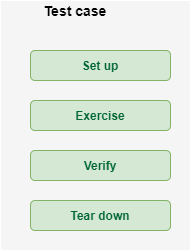
\includegraphics[width=0.5\linewidth]{./testcase.png}
  \caption{Test case}
  \label{fig:testcase}
  \end{center}
\end{figure}
La Figure \ref{fig:testcase}   montre les quatre étapes d'un cas de test unitaire. On distingue:
\begin{itemize}
    \item \textbf{\textcolor{red}{Set up.}} consiste à  préparer les ressources pour le tests;
    \item \textbf{\textcolor{red}{Exercise.}} consiste à exercer la fonctionnalité à tester du  système en tests  sur les ressources précédemment préparées;
    \item \textbf{\textcolor{red}{Verify.}} Consiste à vérifier que le résultat de l'exercice correspond bien au résultat attendu du système en test;
    \item \textbf{\textcolor{red}{Tear down.}} Consiste à libérer les ressources utiliser durant le test
\end{itemize}

\subsubsection{Caractéristiques d'un bon cas test unitaire}
\begin{itemize}
    \item Répétable
\item Pas d'intervention humaine
\item S'auto-décrit
\item Change moins souvent que le système
\item Raconte une histoire
\end{itemize}
\section{Power unit}
\subsection{Présentation}
 \begin{figure}[!htbp]
  \begin{center}
  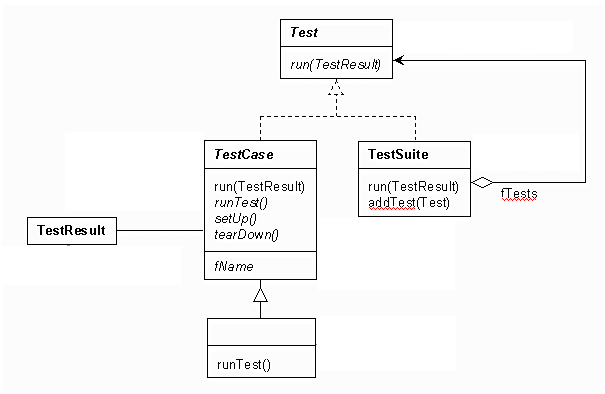
\includegraphics[width=.8\linewidth]{./frameworkPBUnit.png}
  \caption{Power unit}
  \label{fig:powerUnit}
  \end{center}
\end{figure}
Power unit est le framework qui permet d'écrire les tests unitaire en Powerbuilder. Il est inspirer de JUnit.
La Figure \ref{fig:powerUnit} presente le diagramme de classe de Power Unit. La classe \textit{\textcolor{red}{TestCase}} est la classe de base pour écrire les tests unitaire en Powerbuilder.  Ainsi tous les tests héritent de la classe  \textit{\textcolor{red}{TestCase}}. 



\section{Ecriture de tests avec Power Unit}
Dans le cadre de ce apprentissage, je vais reprendre l'exemple de la documentation de Power Unit.
Le programme que nous allons parcourir résoudra le problème de la représentation de l'arithmétique avec des monnaies multiples. 
 L'arithmétique entre les même monnaies  est triviale ; vous pouvez simplement additionner les deux montants.
 Les choses deviennent plus intéressantes une fois que des monnaies multiples sont introduites. 
 Vous ne pouvez pas vous contenter de convertir une monnaie en une autre pour faire de l'arithmétique puisqu'il n'y a pas de taux de conversion unique.

\subsection{Préparation de l'environnement}
Pour suivre ce apprentissage, vous avez besoin:
\begin{itemize}
    \item d'avoir l'IDE \textbf{Powerbuilder} installer sur votre machine
    \item de télécharger les bibliothèques de base ( \textcolor{red}{\textbf{\textit{powerunit.pbl, powerunitfunc.pbl}}} ) de  Power Unit  \href{https://github.com/mahugnon/PowerUnitHonore.git}{ ici} 
    \item de télécharger les bibliothèques de l'interface graphique de Power Unit  \textcolor{red}{\textbf{\textit{powerUnit.zip}}}  \href{https://github.com/mahugnon/PowerUnitHonore/releases/download/v3.1.2/powerUnit.zip}{ici} 
    \item Créer un répertoire qui va accueillir les objets durant ce apprentissage  
    \item Créer un nouvel espace de travail nommé \textit{PBCookBook} 
    \item Copier les bibliothèques ( \textcolor{red}{\textbf{\textit{powerunit.pbl, powerunitfunc.pbl}}}  dans l'espace de travail.
    \item Créer une \textit{target} nommée \textit{PBCookBook} dans l'espace de travail.
    \item Ajouter les bibliothèques ( \textcolor{red}{\textbf{\textit{powerunit.pbl, powerunitfunc.pbl}}}  téléchargée précédemment à la target  .
    \item  Creér une nouvelle bibliothèque PBCookBookTests pour acceuillir les tests.
\end{itemize}

 %\menu{File>Save} or pressing \keys{Ctrl+S}.
\subsection{Creation d'un objet à tester}
Nous allons commencer par définir simplement un objet  qui représentera une valeur monétaire dans une monnaie unique. 
Mais d'abord, créons un objet de base que nous expliquerons plus loin dans ce mode opératoire:
\begin{itemize}
    \item Créer un nouvel objet de classe \textit{custom class}
    \item Fermez et enregistrez-le sous le nom n\_cst\_MoneyBase dans le PBCookBook.PBL
\end{itemize}
Maintenant, créons l'objet monnaie \textit{money}:
\begin{itemize}
   \item Héritez un nouvel objet de l'objet n\_cst\_MoneyBase
    \item Enregistrez le sous le nom de n\_cst\_Money dans la bibliothèque PBCookBook en lui donnant un commentaire approprié
    \item  Définir deux attributs privés pour la somme et la monnaie \textit{money}

\begin{lstlisting}[language=Python, caption=variable d'instance de n\_cst\_money]
    
        Private Decimal	idc_Amount;
        Private String	is_Currency;

\end{lstlisting}
\item Créer une méthode d'initialisation pour ces attributs lors de leur création

\begin{lstlisting}[language=Python, caption=methode d'initialisation  de n\_cst\_money]
    
    /*	of_Initialize ( decimal adc_Amount, string as_Currency )	*/
    idc_Amount = adc_Amount;
    is_Currency = as_Currency;
    return;
\end{lstlisting}
\item  Créer des accesseurs pour les attributs
\begin{lstlisting}[language=Python, caption=accesseur pour recuperer la somme de l'objet \textit{money}]
    
    /*	of_getAmount (): decimal	*/
return	idc_Amount;

\end{lstlisting}
\begin{lstlisting}[language=Python, caption=accesseur pour recuperer la monnaie de l'objet \textit{money}]
    /*	of_getCurrency ( ): String		*/
    return	is_Currency;
    
\end{lstlisting}
\item  Créez une méthode simple pour ajouter les valeurs de deux objets \textit{money} de la même monnaie et obtenir ainsi un nouvel objet \textit{money}.
\begin{lstlisting}[language=Python, caption=Simple addition de deux montants de la même monnaie]
  /*	of_add(n_cst_money anv_Money):n_cst_Money	*/
n_cst_Money	lnv_Money;

lnv_Money = CREATE n_cst_Money;
lnv_Money . of_Initialize ( THIS.of_getAmount() + anv_Money.of_getAmount(), THIS.of_getCurrency( ));
return	lnv_Money;

\end{lstlisting}
\item Avant de pouvoir procéder, nous avons besoins comparer deux objets \textit{money}.  
Ajoutez une nouvelle méthode of\_Equals() à votre objet \textit{n\_cst\_Money}.
 Deux objets Monnaie sont considérés comme égaux s'ils ont la même monnaie et la même valeur
 
 \begin{lstlisting}[language=Python, caption=Comparaison de deux objets \textit{money}]

 /*	of_equals(n_cst_Money anv_Money):Boolean	*/

 IF IsValid ( anv_Money ) THEN
     return (( anv_Money.of_getAmount() = idc_Amount ) &
         AND ( anv_Money.of_getCurrency() = is_Currency ));
 ELSE
     return false;
 END IF;
 
\end{lstlisting}
\end{itemize}

\subsection{Première entrée de jeu}
\subsubsection{Création d'un cas de test}
Maintenant, au lieu de continuer à coder, arrêtons nous et obtenons un retour d'information immédiat en pratiquant 
\textit{\textcolor{red}{"coder un peu, tester un peu, coder un peu, tester un peu"}}.
Un test est mis en oeuvre  en créant une sous-classe de l'objet TestCase.
Nous allons donc créer une classe \textit{n\_cst\_MoneyTest}, que nous allons  placer dans bibliothèque  \textit{PBCookBookTests}.  
Notez que "e" représente le code de la monnaie pour l'euro.
\begin{itemize}
    \item Assurez-vous que le \textit{PBUnit.PBL} figure dans la liste des bibliothèques de votre cible PBCookBook. 
     Cela vous donne accès à toutes les classes d'objets de test PBUnit.
    \item Héritez de la classe TestObject dans PBUnit.PBL et enregistrez-la sous le nom de \textit{n\_cst\_MoneyTest}.
    \item Écrivons un scénario de test pour nous assurer que la méthode \textit{of\_Equals} fonctionne lorsque les objets \textit{money} sont le même objet:
  
 \begin{lstlisting}[language=Python, caption=Test d'égalité de deux \textit{money}]

     /*	EVENT	TestEquals()	*/

n_cst_Money	lnv_euro12;
n_cst_Money	lnv_euro14;
n_cst_Money	lnv_euro12b;

lnv_euro12 = CREATE n_cst_Money;
lnv_euro14 = CREATE n_cst_Money;
lnv_euro12b = CREATE n_cst_Money;

lnv_euro12.of_Initialize( 12.00, "e" );
lnv_euro14.of_Initialize( 14.00, "e" );
lnv_euro12b.of_Initialize( 12.00, "e" );

THIS.Assert ( lnv_euro12.of_Equals ( lnv_euro12 ) );
THIS.Assert ( NOT lnv_euro12.of_Equals ( lnv_euro14 ) );
THIS.Assert ( lnv_euro12.of_Equals ( lnv_euro12b ) );
return
\end{lstlisting}
\item Ajoutez une méthode, \textit{testSimpleAdd()} qui testera notre méthode  \textit{of\_add()}.

\begin{lstlisting}[language=Python, caption=Test d'addition de deux \textit{money}]
    /*	EVENT	testSimpleAdd()	*/
    //		#1
    n_cst_money	lnv_euro12;
    n_cst_money	lnv_euro14;
    n_cst_money	lnv_ExpectedResult;
    n_cst_money	lnv_ActualResult;
    
    lnv_euro12 = CREATE n_cst_Money;
    lnv_euro12.of_Initialize ( 12.00, "e" );
    
    lnv_euro14 = CREATE n_cst_Money;
    lnv_euro14.of_Initialize ( 14.00, "e" );
    
    lnv_ExpectedResult = CREATE n_cst_Money;
    lnv_ExpectedResult.of_Initialize ( 12.00+14.00, "e" );
    //		#2
    lnv_ActualResult = lnv_euro12.of_Add ( lnv_euro14 );
    //		#3
    THIS.Assert ( ( lnv_ExpectedResult.of_Equals ( lnv_ActualResult ) ), true );
    return;
\end{lstlisting}
Maintenant que nous avons créé nos deux cas de test, nous remarquons qu'il y a un peu de duplication de code pour la mise en place de ces deux tests. 
 Il serait bon de réutiliser une partie de ce code de mise en place. 
 Pour ce faire, il suffit de déclarer les objets ressources comme variables d'instance et de les initialiser en redéfinissant l'événement \textit{\textbf{\textcolor{red}{setUp}}}.
 L'opération symétrique de \textit{\textbf{\textcolor{red}{setUp}}}  est le \textit{\textbf{\textcolor{red}{tearDown}}} que vous pouvez redéfinir pour liberer les ressources  à la fin d'un test. 
 Chaque test a ces propre ressources ou son contexte d'execution. \textit{PBUnit}  execute les évènements \textit{\textbf{\textcolor{red}{setUp}}} et \textit{\textbf{\textcolor{red}{tearDown}}}
 pour chaque test pour éviter les éffets de bord au niveau des tests.
 
 \begin{lstlisting}[language=Python, caption=Setup et TearDown]
    Private:
    n_cst_Money	inv_euro12;
    n_cst_Money	inv_euro14;
    
    /*	EVENT	setUp ()		*/
    inv_euro12 = CREATE n_cst_Money;
    inv_euro14 = CREATE n_cst_Money;
    inv_euro12.of_Initialize( 12.00, "e" );
    inv_euro14.of_Initialize( 14.00, "e" );
    
    /*	EVENT	tearDown()	*/
    IF IsValid ( inv_euro12 ) THEN 	DESTROY inv_euro12; 
    IF IsValid ( inv_euro14 ) THEN 	DESTROY inv_euro14;
    
\end{lstlisting}
Nous pouvons réécrire les deux méthodes de cas de test, en supprimant le code de configuration commun :

\begin{lstlisting}[language=Python, caption=Test d'egalité sans la logique du d'initialisation]
    /*	EVENT	TestEqual		*/
    n_cst_Money	lnv_euro12b;
    
    lnv_euro12b = CREATE n_cst_Money;
    lnv_euro12b.of_Initialize( 12.00, "e" );
    
    THIS.Assert ( inv_euro12.of_Equals ( inv_euro12 ) );
    THIS.Assert ( NOT inv_euro12.of_Equals ( inv_euro14 ) );
    THIS.Assert ( inv_euro12.of_Equals ( lnv_euro12b ) );
    return
    
\end{lstlisting}


\begin{lstlisting}[language=Python, caption=Test d'ajout simple sans la logique du d'initialisation]
    /*	EVENT	testSimpleAdd		*/
    n_cst_money	lnv_ExpectedResult;
    n_cst_money	lnv_ActualResult;
    
    lnv_ExpectedResult = CREATE n_cst_Money;
    lnv_ExpectedResult.of_Initialize ( 12.00+14.00, "e" );
    //		#2
    lnv_ActualResult = inv_euro12.of_Add ( inv_euro14 );
    //		#3
    THIS.Assert ( ( lnv_ExpectedResult.of_Equals ( lnv_ActualResult ) ) );
    
    return;
    
    
\end{lstlisting}

\end{itemize}
\subsection{Exécution des tests}
Il existe deux méthodes pour exécuter les tests que vous avez programmés dans votre objet TestCase:  Statique et dynamique.
 Avec la méthode statique, vous surchargerez l'événement runTest dans le n\_cst\_MoneyTest et exécuterez chacun des tests que vous voulez exécuter.


\begin{lstlisting}[language=Python, caption= Redefinition de l'evènement \textit{runTest}]
    /*	EVENT	runTest ()	*/
    THIS. EVENT testEqual ();
    THIS. EVENT testSimpleAdd ();
    Return;
\end{lstlisting}
La méthode dynamique est bien plus pratique que la méthode statique, même si elle permet d'obtenir le résultat souhaité, à savoir l'exécution des deux tests. 
 Avec la méthode statique, vous devez vous souvenir de modifier la méthode \textit{runTest()} pour exécuter tout nouveau test que vous ajoutez à l'objet.
 Avec la méthode dynamique, au lieu de déclarer les tests comme des fonctions d'objet, vous les déclarez comme des \textbf{\textit{\textcolor{red}{EVENTS}}} d'objet qui ne prennent aucun argument et dont le nom commence par \textbf{\textit{\textcolor{red}{"test"}}}.
 C'est pourquoi nous avons utilisé des événements et nommé nos méthodes de test \textit{"testequal"} et \textit{"testsimpleadd"}.
   En ne remplaçant pas l'événement runtest dans notre objet \textit{n\_cst\_MoneyTest}, tous les événements dont le nom commence par  \textbf{\textit{\textcolor{red}{"test"}}} seront automatiquement exécutés.

\subsection{Explication de l'interface graphique de PowerUnit}
Cette partie suppose que vous avez déjà télécharger l'interface de Power  Unit. Si ce n'est pas encore fait, veillez le télécharger \href{https://github.com/mahugnon/PowerUnitHonore/releases/download/v3.1.2/powerUnit.zip}{ici} .
\begin{itemize}
    \item  Extraire le  fichier télécharger  vers "bureau/powerUnit"
    \item  Double cliquer sur \textbf{\textit{\textcolor{red}{powerunitgui.exe}}}. 
    La fenêtre de la Figure \ref{fig:emptyPowerUnit} s'ouvre
    \begin{figure}[!htbp]
        \begin{center}
        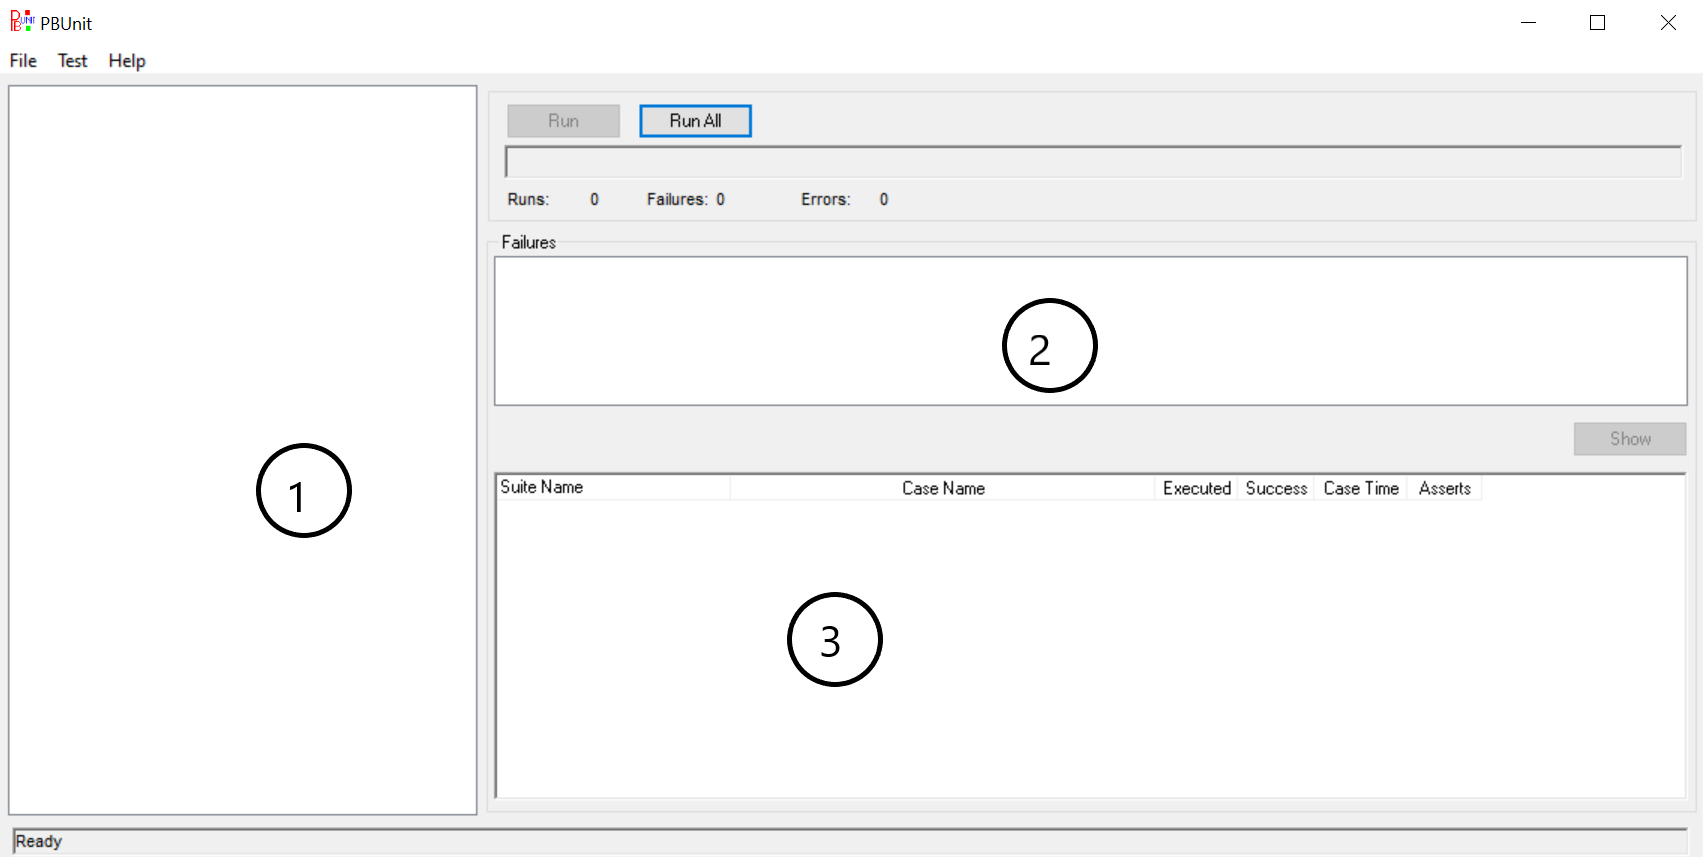
\includegraphics[width=.8\linewidth]{./emptyPowerUnit.png}
        \caption{Power unit}
        \label{fig:emptyPowerUnit}
        \end{center}
      \end{figure}
   L'interface de Power Unit est composée de 3 partie principales.
 La partie (1) presente la liste des tests groupées par les objet \textit{testcase}  contenues dans la \textit{target} sélectionnée.
Parlant de \textit{target}, sélectionnons notre target \textit{PBCookBook.pbt}.
\item  Dans le menu faire \menu{File>Open Target ...} comme indiquer sur la Figure \ref{fig:openTarget} ou bien faite \keys{Ctrl+O}.

\begin{figure}[!htbp]
    \begin{center}
    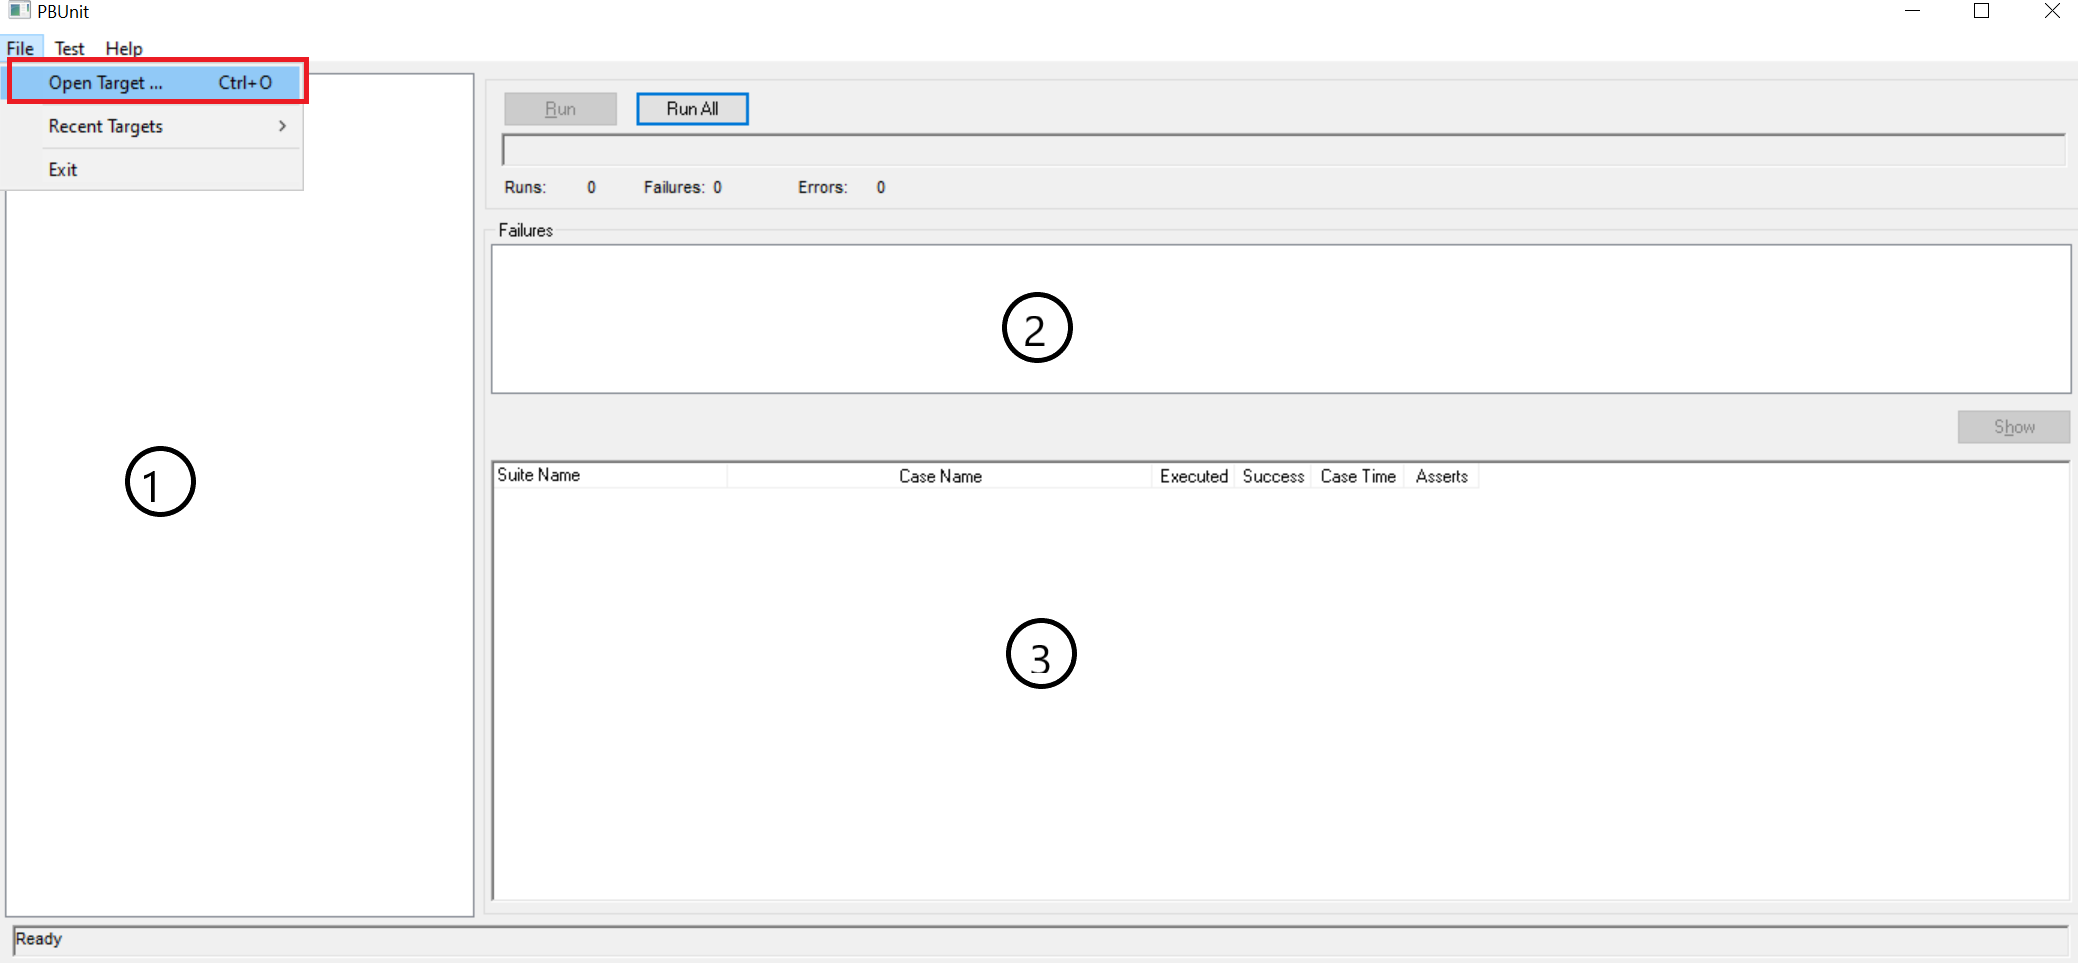
\includegraphics[width=.8\linewidth]{./openTarget.png}
    \caption{Choisir une target}
    \label{fig:openTarget}
    \end{center}
  \end{figure}

  \item  Naviguer vers l'emplacement de la target qui contient les tests (dans ce cas \textit{PBCookBook}), puis selectionner la target \textit{nom\_target.pbt} (\textit{PBCookBook.pbt} dans ce cas). 

  \begin{figure}[!htbp]
    \begin{center}
    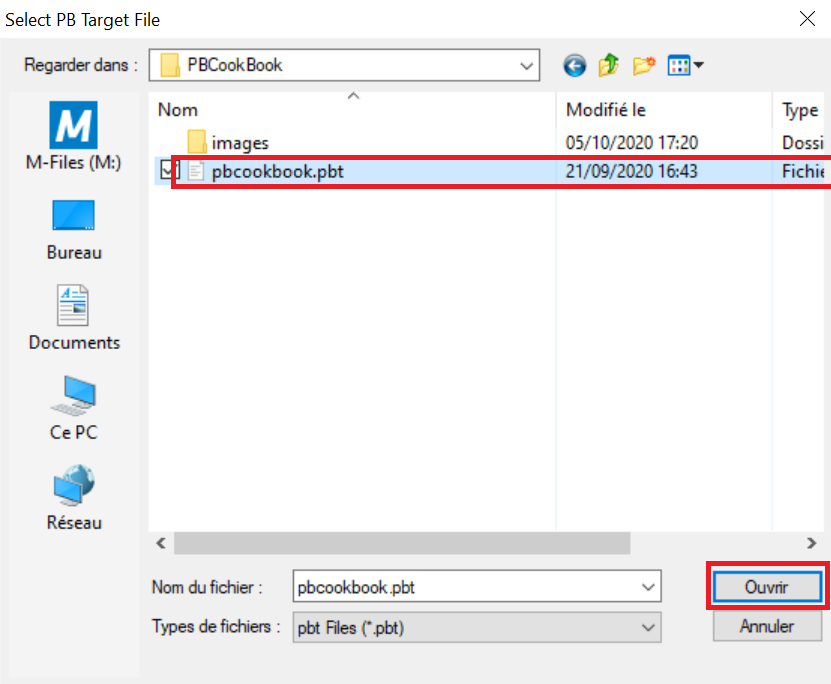
\includegraphics[width=.8\linewidth]{./chooseTestTarget.png}
    \caption{Selectionner la target à son emplacement}
    \label{fig:chooseTestTarget}
    \end{center}
  \end{figure}

  \item  La Figure \ref{fig:afterloadTarget} montre la partie (1) de PowerUnit après chargement des tests.
  \begin{figure}[!htbp]
    \begin{center}
    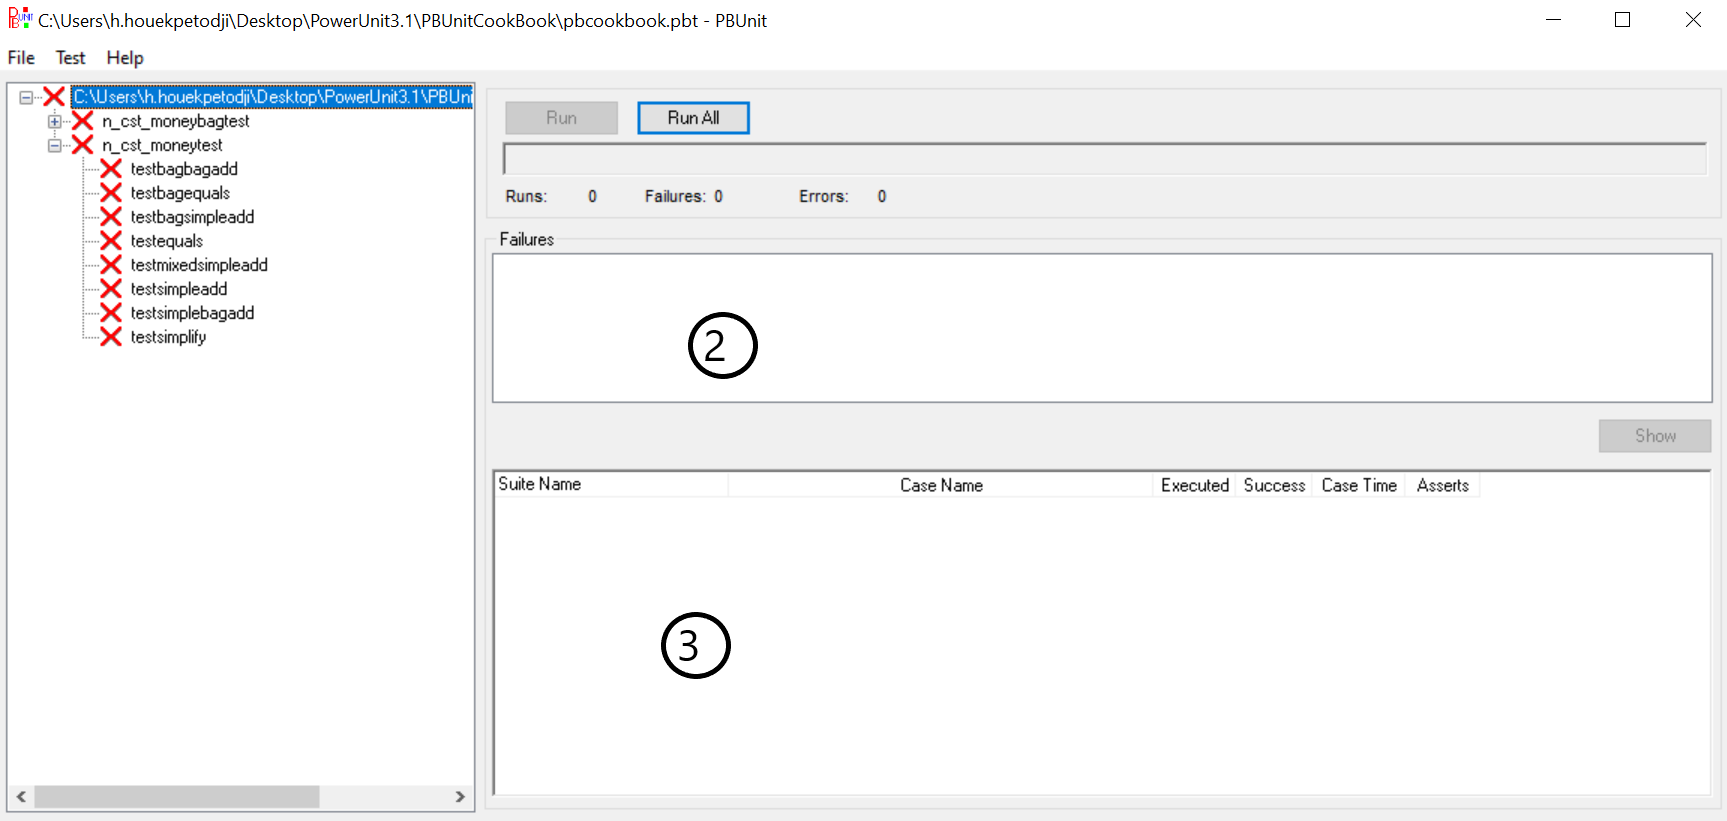
\includegraphics[width=.8\linewidth]{./afterloadTarget.png}
    \caption{PowerUnit après chargement des tests}
    \label{fig:afterloadTarget}
    \end{center}
  \end{figure}
  \item  Selectionner un test et cliquer sur \textit{\textbf{\textcolor{red}{run}}} ou bien cliquer sur \textit{\textbf{\textcolor{red}{runAll}}}
 La Figure \ref{fig:powerUnitTestRunned} présente PowerUnit après exécution des tests.
  \begin{figure}[!htbp]
    \begin{center}
    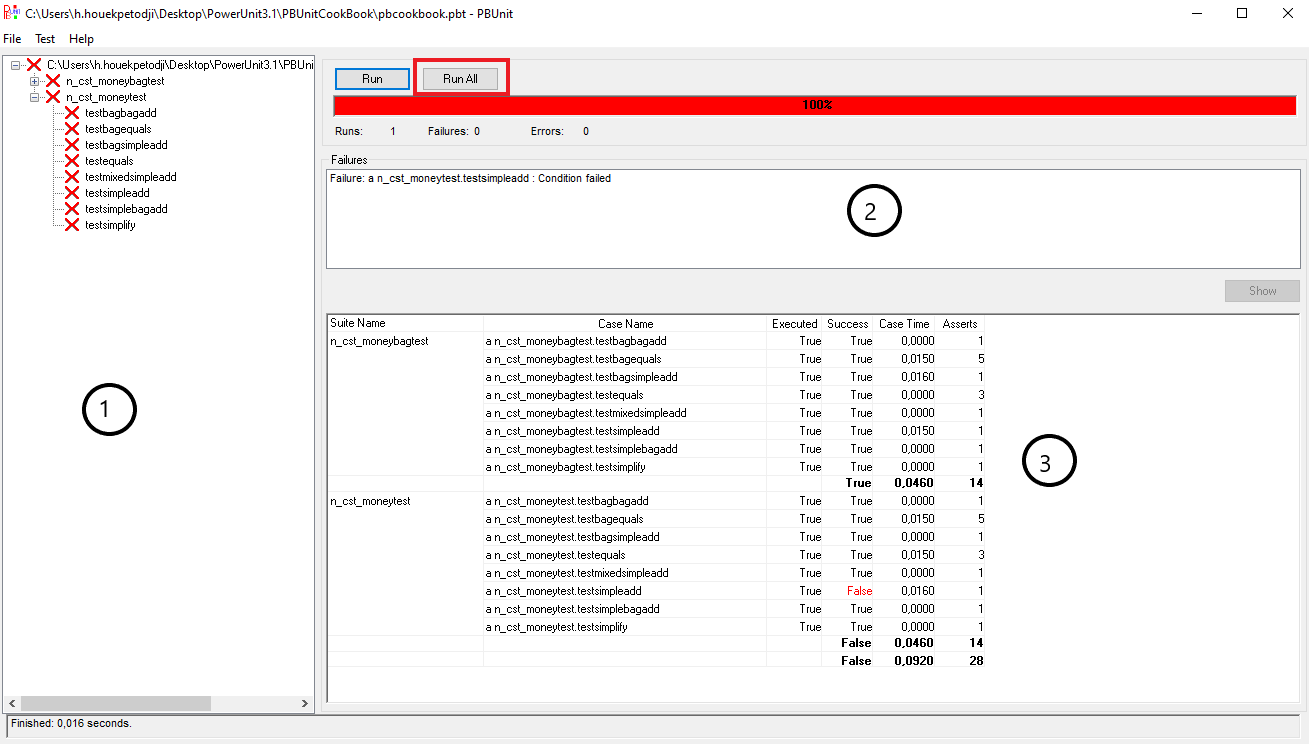
\includegraphics[width=.8\linewidth]{./powerUnitTestRunned.png}
    \caption{PowerUnit après exécution des tests}
    \label{fig:powerUnitTestRunned}
    \end{center}
  \end{figure}
  \item  La partie (2) présente l'ensembe des tests qui ont échoué et la raison de l'échec.
  \item La partie (3) présente  un rapport des executions, l'etat, le temps d'execution, etc.
Dans le cas où tous les tests passent, Power Unit ressemble à la Figure \ref{fig:testPassed}
\begin{figure}[!htbp]
    \begin{center}
    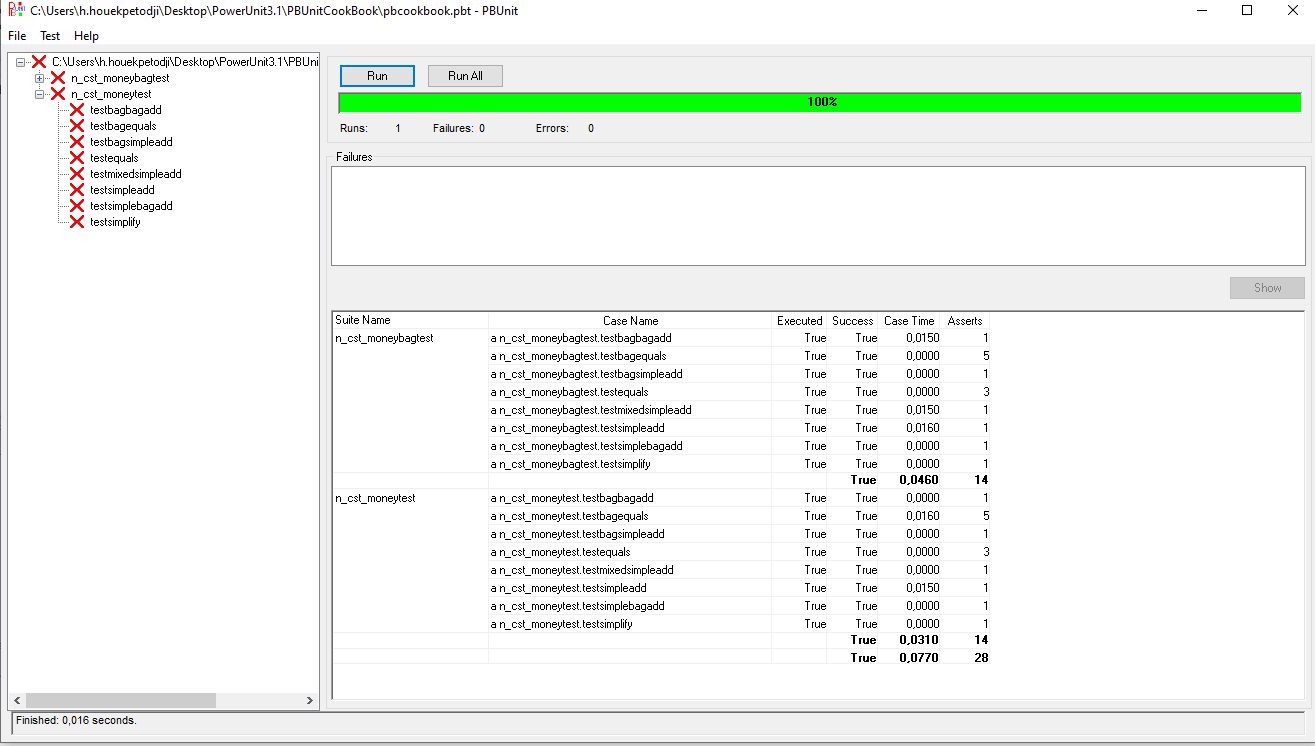
\includegraphics[width=.8\linewidth]{./testPassed.png}
    \caption{PowerUnit après exécution des tests}
    \label{fig:testPassed}
    \end{center}
  \end{figure}
\end{itemize}

\subsection{Integration de PowerUniti avec Izy Protect}
Dans cette section nous allons nous exercer a écrire un test unitaire Pour Izy Protect.
La fonction \textit{f\_decimal} est une fonction gloabale de \textit{Izy Protect} qui prend en paramètre une chaîne de charactère et retourne une valeur décimal.
Elle sera notre candidat pour cet exercice. 
   Pour cela:
\begin{enumerate}
    \item Ouvrir Izy Protect dans L'IDE Powerbuilder
    \item Cliquer droit sur la taget et choisir l'option \textit{Library list...} comme sur la Figure~\ref{fig:librarylist}
    \begin{figure}[!htbp]
        \begin{center}
        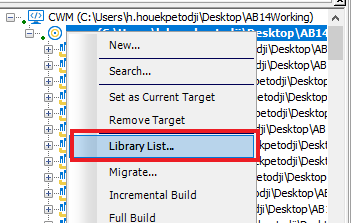
\includegraphics[width=.8\linewidth]{./librarylist.png}
        \caption{Ouvrir la liste des bibliothèques}
        \label{fig:librarylist}
        \end{center}
      \end{figure} 
Ceci ouvrira l'explorateur de Windows qui vous permettra de Naviguer jusqu'à l'emplacement des bibliothèques \textcolor{red}{\textit{\textbf{pbunit et pbunitfunc}}}. 
Si vous ne les retrouver pas, veillez les télécharger \href{https://github.com/mahugnon/PowerUnitHonore.git}{ ici} .
\textbf{\textcolor{red}{ De préference copier ces deux bibliothèques dans la racine de Izy Protect}}. 
Cela facilitera automatisation des execution sur la CI (Jenkins à l'arvenir).
\item Choisir les bibliothèques \textcolor{red}{\textit{\textbf{pbunit et pbunitfunc}}}, puis valider votre choix.
\begin{figure}[!htbp]
    \begin{center}
    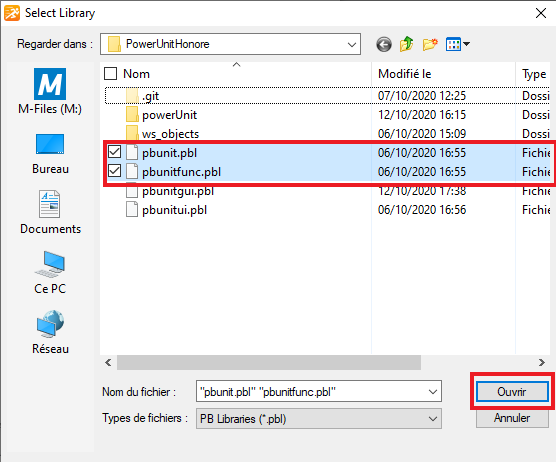
\includegraphics[width=.8\linewidth]{./choosetestbaselibraries.png}
    \caption{Ajouter les bliothèques \textcolor{red}{\textit{\textbf{pbunit et pbunitfunc}}} à Izy Protect}
    \label{fig:librarylist}
    \end{center}
  \end{figure} 
  A cet point on est prêt pour écrire notre premier test unitaire pour Izy Protect. Je nous féllicite \smiley. 
\item  Créer une bliothèque pour acceuillir les test.
 Moi je l'appelle \textit{izy\_protect\_tests} (voir la Figure~\ref{fig:createTestLibrary}).
\begin{figure}[!htbp]
    \begin{center}
    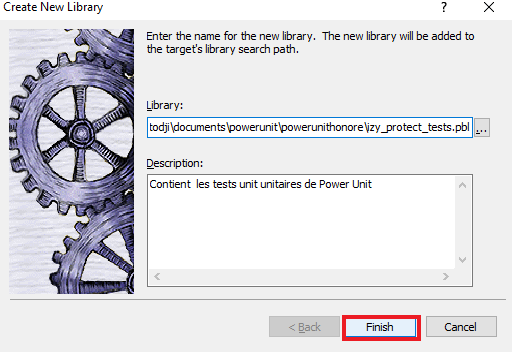
\includegraphics[width=.8\linewidth]{./createTestLibrary.png}
    \caption{Bibliothèque de tests}
    \label{fig:createTestLibrary}
    \end{center}
  \end{figure} 
  \item Faire  \menu{pbunit.pbl>testcase}, puis cliquer droit sur \textit{testcase}  et faire  \menu{testcase>Inherit from}.
  \item Nommer l'object test \textit{test\_f\_decimal} et chosir la bibliothèque de test comme sur la Figure~\ref{fig:nameTestObject}
  \begin{figure}[!htbp]
    \begin{center}
    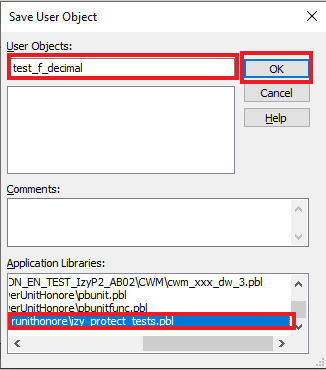
\includegraphics[width=.8\linewidth]{./nameTestObject.png}
    \caption{Enregister la testcase}
    \label{fig:nameTestObject}
    \end{center}
  \end{figure} 
A titre de rappelle, un test cas de test unitaire est de préférence un evènement  qui ne retourne rien. 
Ceci étant allons-y créer un test pour notre function gloable \textit{f\_decimal}.
\item Créer deux évènements
\begin{lstlisting}[language=Python, caption= f\_decimal test 1]
    /*	EVENT	test\_integerString\_to\_decimal ()	*/
    this.assertEqual(f\_decimal('12'),12.00)
\end{lstlisting}

\begin{lstlisting}[language=Python, caption= f\_decimal test 2]
    /*	EVENT	test\_decimalString\_to\_decimal ()	*/
    this.assertEqual(f\_decimal('0.45127'),0.45127)
\end{lstlisting}
\item  Faire \menu{File >Open Target ..} ou bion \keys{Ctrl+O} puis choisir la \textit{target.pbt} de \textit{Izy Protect} et valider.
\item Cliquer sur le bouton \keys{runAll} pour executer les deux tests. La Figure~\ref{fig:testPass} montre le result. 
\begin{figure}[!htbp]
    \begin{center}
    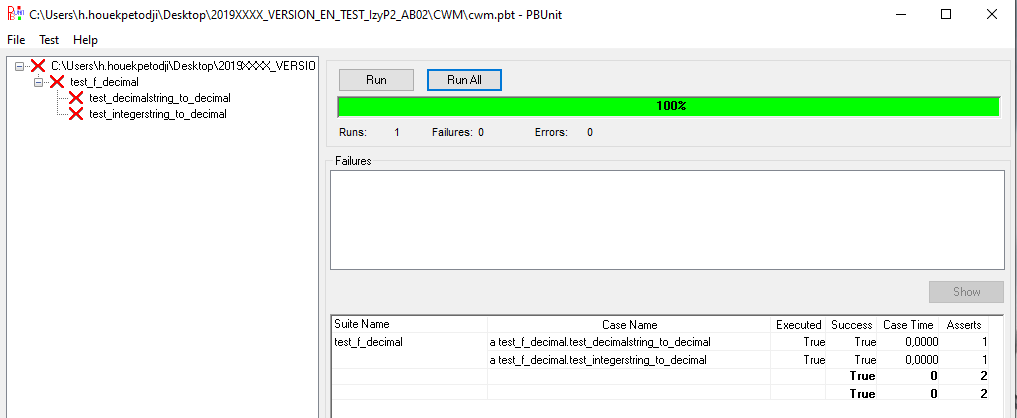
\includegraphics[width=.8\linewidth]{./uf_decimal_tests_pass.png}
    \caption{Executer les tests de f\_decimal}
    \label{fig:testPass}
    \end{center}
  \end{figure}
  Pour aller plus loin, on pourrait tests d'autres aspect de \textit{f\_decimal}. 
  Par exemple qu'est-ce qui se passe si on a \textit{f\_decimal("abc15")}?
 Je vous laisse le soin d'essayer ça.
  J'ai pas la réponse \smiley.
\end{enumerate}
  
\newpage
Je vous remercie, \textbf{HOUEKPETODJI Mahugnon Honoré}
% \bibliographystyle{plain}
% \bibliography{refs}
\end{document}